\section{Results}
\label{sec:results}

\begin{table*}[t]
\centering\small
\setlength{\tabcolsep}{3.6pt}
\begin{tabular}{@{}lrlcccccccc@{}}
\toprule
Doc & Sent. & Annotated by & Zero-shot & Seed $H_0$ & Learned & $\Delta$ F & Seed & Learned & $\Delta$ C & Trained \\
 & & & prompt F & F & F & & C & C & & on it, F \\
\midrule
0001 & 51 & $H_{0}$ & 31.0 & 45.1 & -- & -- & 40.5 & -- & -- & 77.5 \\
0002 & 60 & $H_{1}$ & 31.1 & 49.4 & 61.1 & +11.8 & 44.1 & 56.2 & +12.1 & 77.3 \\
0003 & 31 & $H_{2}$ & 32.3 & 45.3 & 57.2 & +11.9 & 41.3 & 55.4 & +14.1 & 84.4 \\
0004 & 59 & $H_{3}$ & 33.5 & 42.9 & 52.4 & +9.5 & 39.3 & 49.7 & +10.4 & 72.4 \\
0005 & 40 & $H_{4}$ & 32.3 & 48.0 & 58.5 & +10.5 & 44.4 & 57.1 & +12.7 & 79.7 \\
0006 & 35 & $H_{5}$ & 23.6 & 49.3 & 56.1 & +6.8 & 40.4 & 49.2 & +8.8 & 81.0 \\
0007 & 82 & $H_{6}$ & 32.6 & 46.4 & 65.5 & +19.1 & 42.3 & 59.6 & +17.3 & 85.4 \\
0008 & 10 & $H_{7}$ & \gapcell{} & 57.1 & 56.4 & $-$0.8 & 52.5 & 53.7 & +1.2 & 92.7 \\
0009 & 10 & $H_{8}$ & \gapcell{} & 59.7 & 68.0 & +8.3 & 55.2 & 65.3 & +10.1 & 99.2 \\
0010 & 12 & $H_{9}$ & \gapcell{} & 51.2 & 55.2 & +4.0 & 45.7 & 50.2 & +4.5 & 92.5 \\
0011 & 25 & $H_{10}$ & \gapcell{} & \gapcell{} & 53.4 & \gapcell{} & \gapcell{} & 48.5 & \gapcell{} & -- \\
\midrule
Mean, 9 paired documents & & & -- & 49.9 & 58.9 & +9.0 & 45.0 & 55.2 & +10.1 & \\
Mean, 0002--0007 & & & 30.9 & 46.9 & 58.5 & +11.6 & & & & \\
\bottomrule
\end{tabular}
\caption{Sequential (test-then-train) evaluation on Chinese UMR. Document $n$ is annotated by the harness built from documents $1..n{-}1$ (``Learned''), then used to improve it. ``Seed'' is $H_0$ on the same document, the paired control. ``Zero-shot prompt'' is one call per sentence with no harness (sentence graph only, so only F is comparable). F = AnCast++ sentence F; C = comprehensive score (sentence graphs plus document-level relations). The last column is the harness trained on the document itself (training fit, not generalization). Document 0001 has no earlier harness; 0011 has no seed run yet; zero-shot is missing for 0008--0011.}
\label{tab:prequential}
\end{table*}


\begin{figure*}[t]
\centering
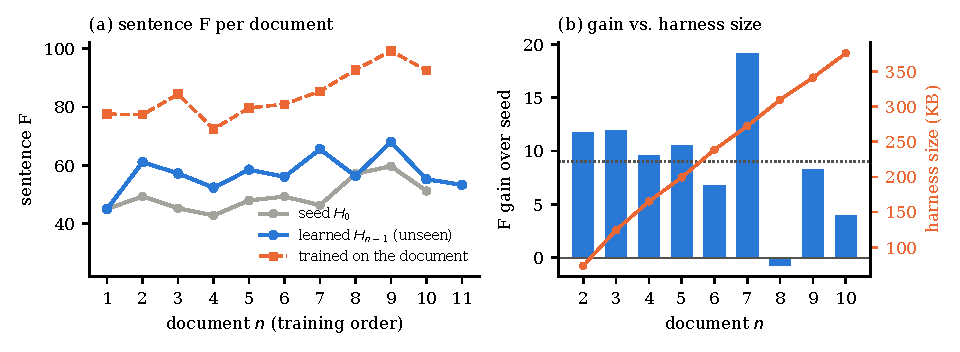
\includegraphics[width=\textwidth]{figures/curve.pdf}
\caption{(a) Sentence F per document in training order: seed harness, learned harness that has not seen the document, and the harness after three rounds on it. (b) Gain of the learned harness over the seed per unseen document (bars; dotted: mean) and the size of the harness that annotated it (line).}
\label{fig:curve}
\end{figure*}

\subsection{The learned harness is better on unseen documents}
\label{sec:main}

On the documents that also have the zero-shot prompt (0002--0007; Table~\ref{tab:prequential}), the systems form a ladder: \zeroMeanZ{} F for one call per sentence, \seedMeanZ{} for the seed harness, \firstMeanZ{} for the learned harness. Over the \nPaired{} documents with a seed control, the learned harness gains \gainF{} F (95\% CI \gainFLo--\gainFHi; Wilcoxon $p=$~\gainFWilcoxon) and improves \gainFPos{} of them; on the comprehensive score it gains \gainC{} (\gainCLo--\gainCHi) and improves all \gainCPos{} ($p=$~\gainCWilcoxon). Of \nSentPaired{} complete-case paired sentences, \sentBetter\% improve and \sentWorse\% decline by more than one Smatch point (mean +\sentGain, \sentGainLo--\sentGainHi). The one document that does not improve, 0008 (\gainMin), has ten sentences.

\paragraph{Training fit is not generalization.}
Three rounds on a document raise its own F by \trainFitGain{} points, to \afterMean{} on average and up to \afterMax, against \gainF{} on the next, unseen document (Figure~\ref{fig:curve}a). The leakage guard restricts some verbatim overlap, not learning one document's particular conventions. Evaluated on its training documents, the same loop would look three times better.

\subsection{Against baselines with the same gold}
\label{sec:baselines}

\begin{table}[t]
\centering\small
\setlength{\tabcolsep}{4pt}
\begin{tabular}{@{}lccr@{}}
\toprule
System (gold: 0001--0004) & F & C & Calls/sent. \\
\midrule
Zero-shot prompt & \gapcell & -- & 1 \\
Few-shot, $k{=}30$ & \gapcell & \gapcell & 3 \\
Guideline-only refinement & \gapcell & \gapcell & 1 \\
Procedural harness & \gapcell & \gapcell & dozens \\
\midrule
Seed harness $H_0$ & \gapcell & \gapcell & 3 \\
Learned $H_4$ (and $H_1$, $H_{10}$) & \gapcell & \gapcell & 3 \\
\bottomrule
\end{tabular}
\caption{Planned held-out set (20 documents not used to train this harness), same gold budget for all trained systems. \gap{G1--G4}}
\label{tab:heldout}
\end{table}

The held-out comparison is pending (Table~\ref{tab:heldout}). One matched comparison exists: trained on 0001--0004 with the same models, the learned harness scores \matchedCrit{} F on document 0005 and the procedural harness \matchedTree{}; the procedural seed starts higher there (\treeSeedFive{} vs.\ 48.0), so the learned gains are +\critGainFive{} and +\treeGainFive{} (one document; the procedural harness had 10 rounds, ours 12; Appendix Table~\ref{tab:matched}).

\subsection{Where the gains come from}
\label{sec:where}

\paragraph{Stage-wise generator and checker scores.}
Scoring the graph after each step (Appendix Table~\ref{tab:critique}) shows that the learned \skill{generate} alone is \genGain{} F better than the seed's on unseen documents, and \skill{critique} adds \critFirst{} on top (\critFirstMin{} to +\critFirstMax), less than the \critSeed{} it adds to the seed's draft; on the document it was trained on it adds \critAfter. Most of the observed sequential gain is already present at the generator stage. These stage-wise comparisons do not isolate the causal contribution of updating each skill, because the generator and checker were revised jointly. A variant with five specialized checks shows this more sharply: the checks add +\refineTrainMin{} to +\refineTrainMax{} on their training documents and \refineUnseen{} on unseen ones (Appendix Table~\ref{tab:refine}). At annotation time a checker has no gold, only what it was told, as self-correction studies would predict \citep{huang2024large,kamoi2024when}.

\begin{figure}[t]
\centering
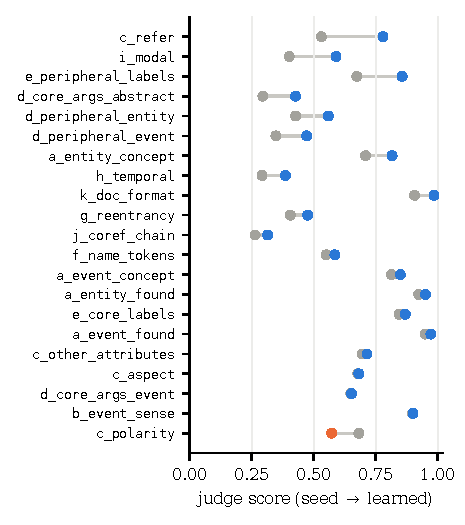
\includegraphics[width=\columnwidth]{figures/category.pdf}
\caption{Judge score per check on unseen documents: seed (grey) and learned harness (blue; orange where lower), mean over \nPaired{} documents.}
\label{fig:category}
\end{figure}

\paragraph{Gains by evaluator check.}
By judge check (Figure~\ref{fig:category}), the largest gains are on the scheme's conventions: pronoun person and number (+\catRefer{} points), the author's modal strength (+\catModal), non-core role labels (+\catPeriph), arguments of abstract rolesets such as \texttt{have-org-role-91} (+\catAbstract), non-core arguments of events (+\catPeriphEvent), entity concepts (+\catEntity). Little change is observed on several checks involving semantic judgments: PropBank sense (+\catSense), aspect (+\catAspect), core arguments of events (+\catCoreEvent). Coreference (+\catCoref) gains little and polarity falls (\catPolarity, few units). This pattern is consistent with learning scheme conventions, but these checks also involve semantic judgments. It does not establish an unchanged semantic capability or a capability ceiling; category counts and repeated, targeted comparisons are needed to test that interpretation.

\subsection{Tools are proposed rarely and admitted never}
\label{sec:tools}

In \nRounds{} rounds the builder proposed \nProposals{} tools and no steps; the reviewer rejected all three. \texttt{check\_umr\_graph} checked attribute values, entity types and role names; the reviewer kept the purely mechanical checks (colon-prefixed or misspelled closed-list values, parse failures, duplicate variables) and judged the rest to be missing conventions that belong in the instructions. \texttt{check\_umr\_form} flagged bare constants and aspect on discourse rolesets; the second part contradicted the builder's own earlier rule. \texttt{check\_doc\_relations} checked coreference on name nodes and double temporal parents, but one test contradicted a convention of \skill{document}. Each time a sound core was lost, because rejected proposals are not revised. Without the reviewer (the TimeML and manifesto runs), the builder changes tools or rules in most rounds \gap{G7: does admitting them help?}.

\subsection{Instruction growth without a clear increase in sequential gains}
\label{sec:growth}

This trajectory shows no clear increase in gain with the number of preceding documents (Figure~\ref{fig:curve}b): +\gainFirstHalf{} on average for documents 2--6, +\gainSecondHalf{} for 7--10 (Spearman $\rho=$~\gainRho, $p=$~\gainRhoP). The harness grows from \sizeSeed{} to \sizeLast{}\,KB (\sizeGen{} in \skill{generate}, \sizeCrit{} in \skill{critique}, \sizeDoc{} in \skill{document}), \sizePerRound{}\,KB per round. Of \nEditsApplied{} applied edits, \nModify{} modify, \nAdd{} add and \nDelete{} delete (Appendix Table~\ref{tab:edits}): nothing rewards a shorter harness. The correlation does not establish a flat learning curve, since document difficulty and order change along with the harness. Whether this pattern reflects what one document can teach, from interference among accumulated rules, or from length is open; held-out scores of $H_1$ to $H_{10}$ and a consolidation pass under a size budget would separate these \gap{G5, G6}.

\begin{table}[t]
\centering\small
\setlength{\tabcolsep}{2pt}
\begin{tabular}{@{}llrrrr@{}}
\toprule
Builder / annotator & Harness & $n$ & Seed & Learned & $\Delta$ \\
\midrule
Opus / Sonnet 5.5 & ours$^s$ & 9 & 49.9 & 58.9 & +9.0 \\
Opus / Sonnet 5.5 & proc. & 2 & 45.5 & 52.9 & +7.4 \\
DeepSeek (no thinking) & proc. & 5 & 32.5 & 37.6 & +5.2 \\
Qwen3.5-9B & proc.$^s$ & 13 & 17.6 & 16.3 & $-$1.4 \\
\midrule
Qwen3.5-27B & proc.$^s$ & \gapcell{} & \gapcell{} & \gapcell{} & \gapcell{} \\
Opus / small model & ours & \gapcell{} & \gapcell{} & \gapcell{} & \gapcell{} \\
Small model / Sonnet & ours$^s$ & \gapcell{} & \gapcell{} & \gapcell{} & \gapcell{} \\
\bottomrule
\end{tabular}
\caption{Seed vs.\ learned harness on unseen documents, sentence F. One name: the same model builds and annotates. proc.: procedural harness. $^s$sequential protocol; otherwise a few training documents and separate test documents. DeepSeek's seed reaches 49.1 F with thinking on vs.\ 35.9 off (document 0002).}
\label{tab:models}
\end{table}


\subsection{A weaker joint builder--annotator configuration}
\label{sec:models}

The gain holds for the procedural harness with the same models and for DeepSeek building and annotating without thinking (Table~\ref{tab:models}). With Qwen3.5-9B building and annotating over \qwenSmallN{} documents, the learned harness is worse than the seed (\qwenSmallGain{} F on average; better on \qwenSmallPos{} documents), and the decline deepens (+\qwenSmallFirst{} in the first half, \qwenSmallSecond{} in the second); two independent seed runs differ by \qwenSeedNoise{} F per document, which limits interpretation of individual changes. The available reruns do not establish the significance of the trajectory. On agentic tasks, by contrast, a 9B model's harness updates were as useful as a frontier model's \citep{lin2026harness}. Whether builder or annotator matters more here is not yet separated \gap{G8}.

\subsection{Ablations of the loop}
\label{sec:ablation}

\begin{table}[t]
\centering\small
\setlength{\tabcolsep}{3pt}
\begin{tabular}{@{}lccc@{}}
\toprule
Variant & $\Delta$F seq. & $\Delta$F held-out & KB \\
\midrule
\sys & \gapcell & \gapcell & \gapcell \\
\quad no attribution (one list) & \gapcell & \gapcell & \gapcell \\
\quad whole-skill rewrites & \gapcell & \gapcell & \gapcell \\
\quad \skill{generate} only & \gapcell & \gapcell & \gapcell \\
\quad no reviewer & \gapcell & \gapcell & \gapcell \\
\quad + test edits on held-in docs & \gapcell & \gapcell & \gapcell \\
\quad + consolidation & \gapcell & \gapcell & \gapcell \\
\quad other document orders & \gapcell & \gapcell & \gapcell \\
\bottomrule
\end{tabular}
\caption{Planned matched-budget ablations: sequential gain on 0002--0005 and gain on the held-out set. All rows must be recomputed on this common protocol; the reported full-run gain over 0002--0010 is not a baseline for this subset. \gap{G9}}
\label{tab:ablation}
\end{table}

Table~\ref{tab:ablation} lists the ablations that test the design: whether attribution to a skill matters (one undivided problem list), whether typed edits matter (each round rewrites a skill in full, as guideline refinement does), whether the checking step is needed, whether the reviewer helps or only blocks, whether testing each edit before keeping it \citep{zhang2026self,kim2026refining} closes the training-fit gap, whether consolidation lifts the plateau, and how much document order matters \gap{G9: to run}.

\subsection{Beyond UMR}
\label{sec:beyond}

The same loop builds a TimeML annotator for TempEval-3 \citep{uzzaman2013semeval} and a coder that assigns manifesto sentences one of the eight policy domains of the Manifesto Project scheme \citep{lehmann2026manifesto}, with variant protocols that omit the model reviewer and permit rule and registry changes (Appendix~\ref{app:other}; finished baselines in Tables~\ref{tab:timeml} and~\ref{tab:manifesto}). On both test sets the seed harness is below the zero-shot prompt (TimeML event F1 74.5 vs.\ 80.7; manifesto accuracy 63.8 vs.\ 65.0), so the learned harness must first make up for its own seed. \gap{G10, G11: learned harness on both test sets; sequential gains.}
